\section{A detailed discussion of the `one-way' approach to estimating the remote resource} \label{appendix:one-way-method}

The one-way approach to estimating $R_r$ deserves some explanation because it deviates from the traditional definition of a line-integral. In a traditional line-integral the directionality coefficient is simply:
\begin{align}
    \delta_{*} = \cos(\theta_n - \theta)
    \label{eqn:trad-def}
\end{align}
The primary problem with this definition for the purposes of wave resource assessment is that waves that propagate away from the shoreline of interest ($|\theta_n - \theta|>90$) are subtracted from the resource total. This motivates consideration of two alternate definitions of $\delta$. First, a `bi-directional' case:
\begin{align}
    \delta_2 = |\delta_{*}|
    \label{eqn:2way-def}
\end{align}
and the one-way case:
\begin{align}
    \delta_1 = 
    \begin{cases}
     \delta_* & \mathrm{for\ }|\theta_n - \theta|<90\ \mathrm{degrees} \\
    0 & \mathrm{otherwise}.       
    \end{cases}
    \label{eqn:1way-def}
\end{align}
In weighing the pros/cons of these definitions of $\delta$ it is important to understand that wave resource assessments are typically based on models that do not extract wave energy when it encounters the integration contour of interest (e.g., $\leez$). That is, wave energy that propagates across the integration contour at one location might propagate across it again at another location, and there is typically no way to `track' waves (i.e., wave energy) within these models.
This means that both of the definitions of $\delta$ in \eqref{eqn:2way-def} and \eqref{eqn:1way-def} will `double-count' waves that criss-cross back-and-forth across the integration countour ($\delta_2$ to a larger degree). This can occur for waves that travel straight across a zig-zagging integration contour, or for waves that zig-zag along a straight contour. 

\begin{figure}[ht]
    \centering
    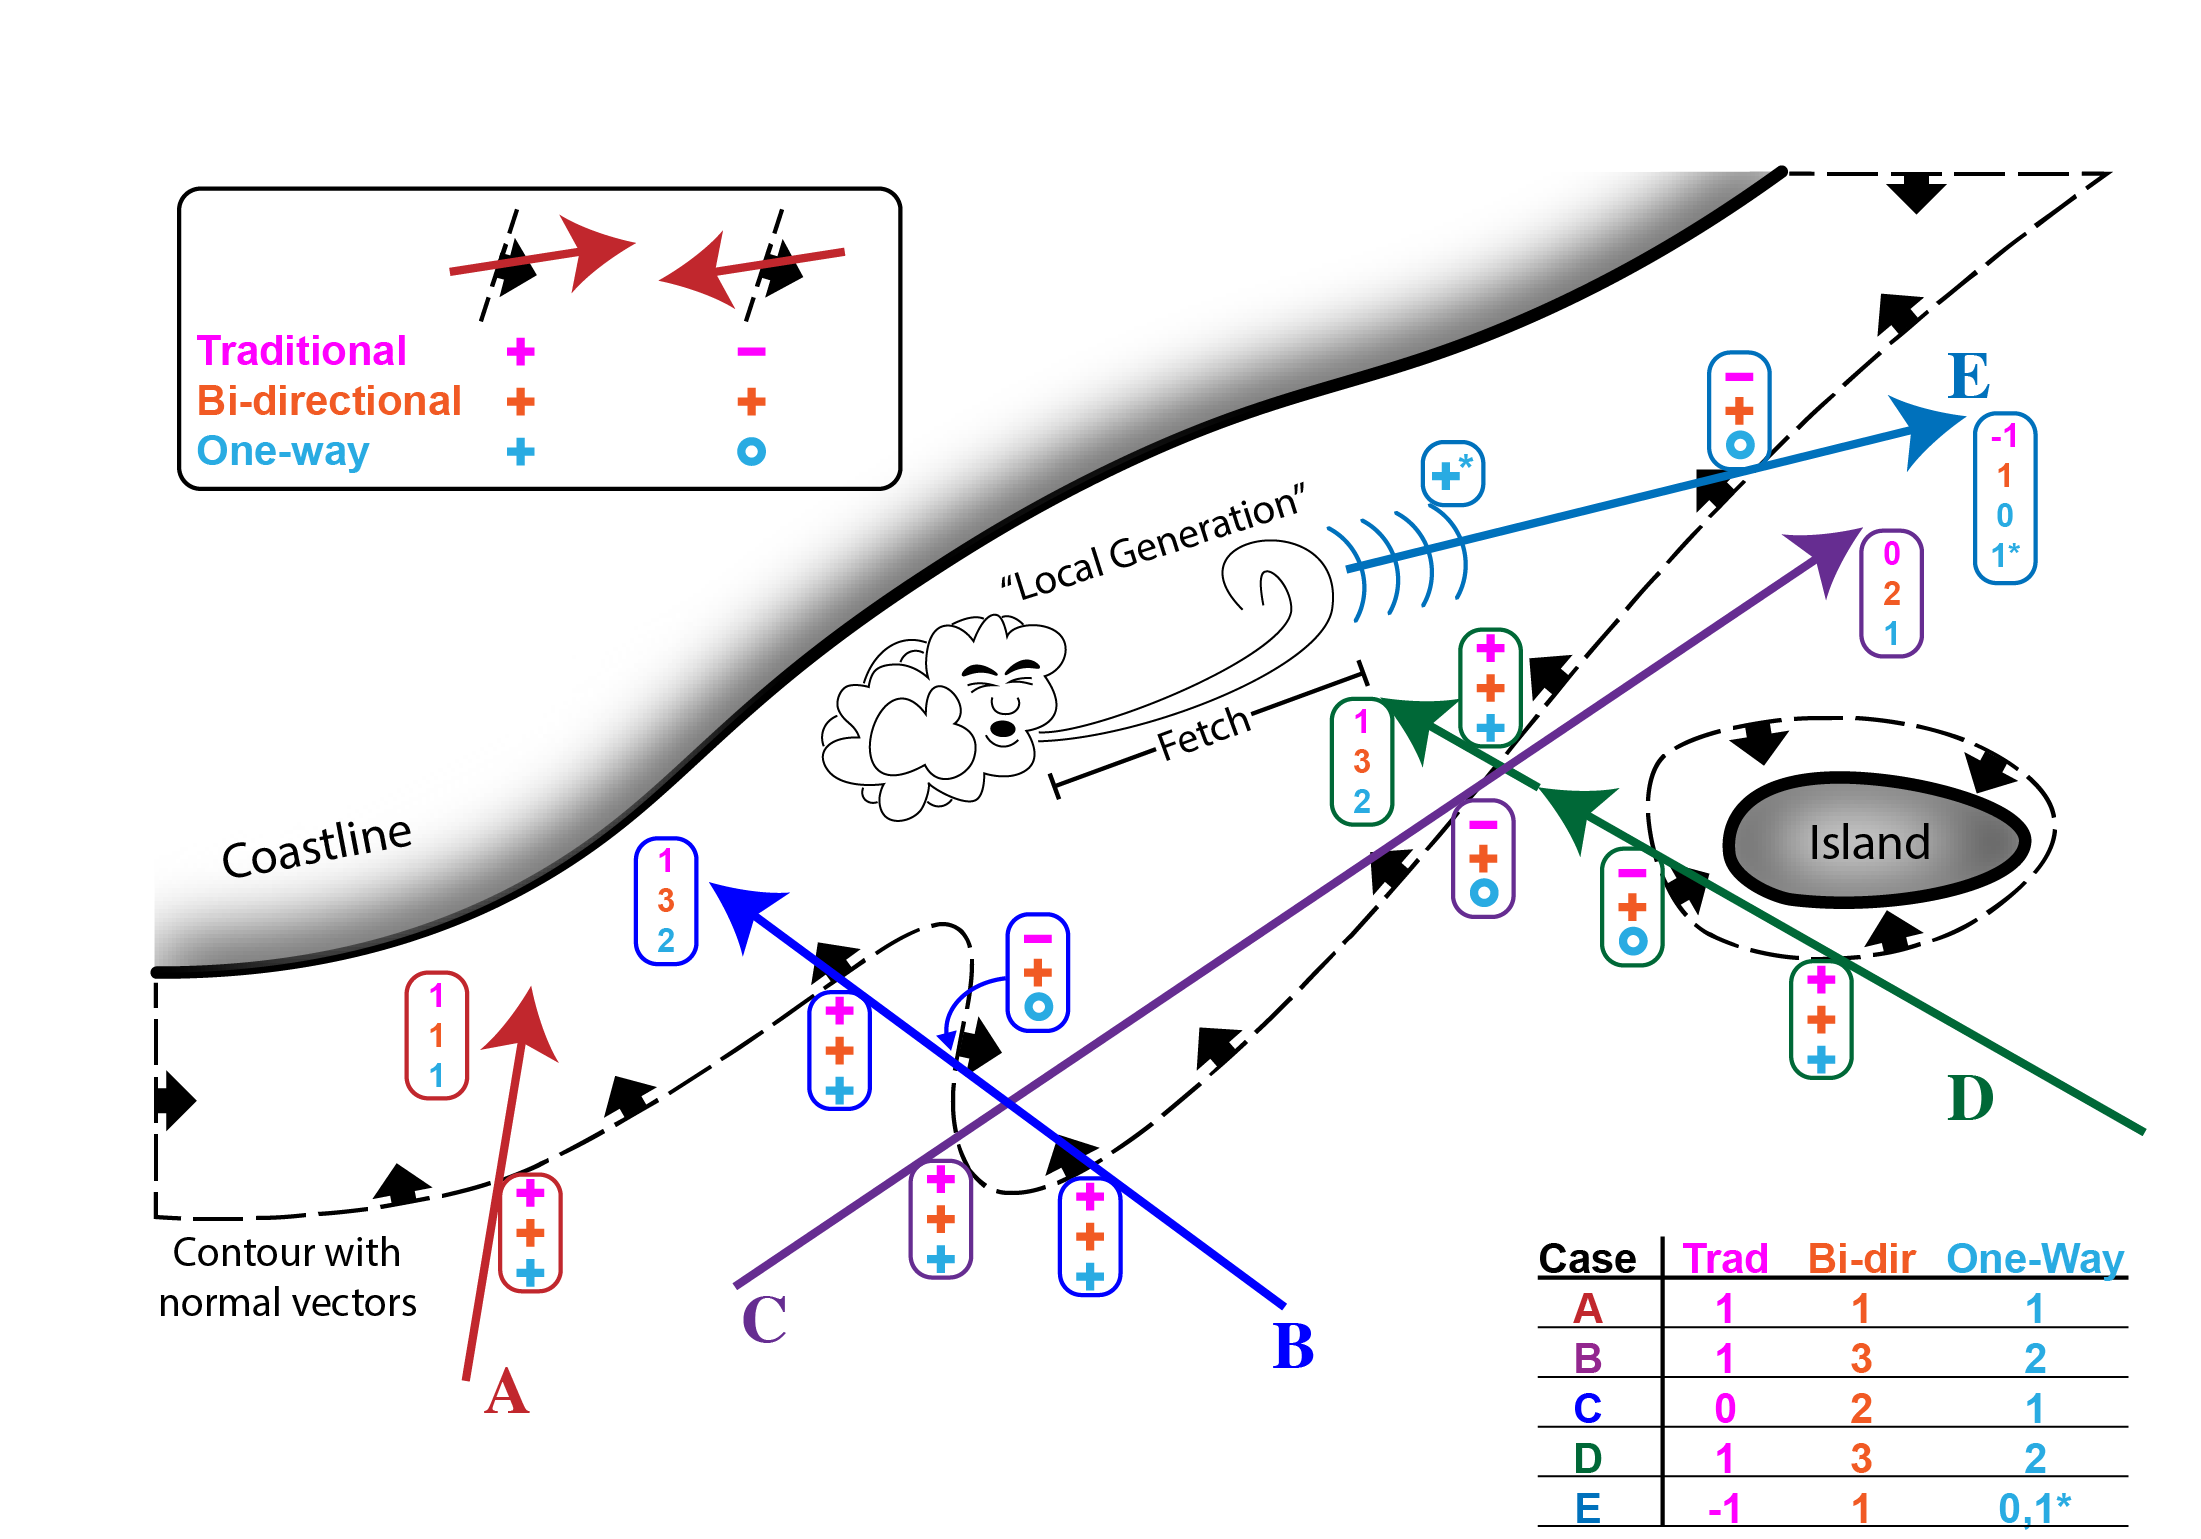
\includegraphics[width=\linewidth]{../diagram/Schematic-Seq01FINAL.png}
    \caption{A diagram depicting different cases of waves (color arrows) crossing an arbitrary integration contour (black dashed line). Black arrows along the contour indicate the contour-normal direction. The upper-left legend — and the boxes along the arrows' lengths — indicate whether energy is added to, subtracted from, or not included in the total depending on the summation method (pink: traditional, orange: bi-directional, cyan: one-way) and direction of wave crossing relative to contour. Boxes at the tip of each arrow indicate the number of times each wave was counted using each method, and the table at lower-right summarizes the totals. A `blowing cloud' image indicates the generation of `local waves' over the region bounded by the integration contour. \note{Need to add a row $E^\dagger$}}
    \label{fig:one-way-diagram}
\end{figure}

Figure \ref{fig:one-way-diagram} provides a schematic of several distinct cases of wave energy (color arrows) propagating across an arbitrary integration contour (black dashed line). Arrow `A' (red) indicates the simplest case of a wave train crossing the contour once before dissipating at the coastline. In this case, all three definitions of $\delta$ give the same correct result of counting this wave exactly once. Arrow `B' (blue) is the case where a wave crosses a zig-zagging countour several times, and shows that $\delta_1$ and $\delta_2$ double-count and triple-count this wave. Arrow `C' (purple) is a case where a wave propagates into and out-of the integration boundary, demonstrating that the $\delta = \delta_*$ does not count this wave, $\delta_1$ counts it once, and $\delta_2$ double-counts it. Arrow `D' (green) is the case of a wave propagating through an island's contour before entering the mainland contour, with essentially the same result as wave `B'. It is also interesting to consider the case where wave `D' does not enter the mainland contour (i.e., if the island is far from shore), in which case the results are the same as wave C.

Finally, this brings us to case `E' where a wave is generated inshore of the boundary and propagates offshore. In this case the wave's energy is subtracted from the total for the traditional case, not counted for the one-way case, and added once (correctly) for the bi-directional method. Note that this is the only case—other than simple case (A)—where the bidirectional method delivers the correct result. When the one-way method is used in conjunction with the local resource method, this waves' energy is included in the total.
When the local resource is added to the numbers in row E, this wave's energy is counted again, which yields row E$^\dagger$.

Importantly, the table in Figure \ref{fig:one-way-diagram} shows that none of the methods defined by the definitions of $\delta$ deliver an accurate estimate of the wave resource for all possible wave paths and integration contours. The only way to avoid double-counting completely is to extract wave energy at the integration contour so that it does not propagate to a different point on the contour where it could be double-counted (or subtracted, depending on the choice of $\delta$). This approach, however, is technically challenging and reduces the flexibility of data analysis (i.e., simulations must be run for each integration contour the user wishes to investigate).

Instead, it is worthwhile to note that $\delta_*$ will always provide a lower-bound estimate of $R_t$, and the bidirectional method will provide an upper-bound estimate. consider which sources of error associated with the definition of $\delta$ are the magnitude of the error associated with each method. 
This means that while using $\delta = \delta_*$ has the potential to underestimate the resource, both 

$\delta = \delta_*$ vs. overestimating the resource using $\delta = \delta_1$ or $\delta_2$ 




In order to do so, it is important to first understand that wave resource assessment is typically conducted using numerical simulations where wave energy models that do not extract energy from the 



In order to address address the national academy of science's 
most important short2011 U.S. wave resource assessment, it is important to account for wave directionality in the The directionality coefficient, $\delta$ Note that this approach does `double count' waves that criss-cross the integration contour ($\leez$ in this case) more than once, but so long as $\leez$ is relatively straight this is generally a small fraction of waves.

This approach, however, can be technically challenging and reduces the flexibility of interpreting results (i.e., simulations must be run for each contour of interest, rather than being able to compute resource totals for different contours from a single simulation). A more detailed justification for the `one-way' approach is provided in appendix \ref{appendix:one-way-method}.

%An estimate of the error associated with the `one-way' condition can be obtained by setting $\delta = 1$ for all directions (i.e., a conventional dot-product). The magnitude of the difference between this estimate of $R_r$ and the one obtained using the one-way condition provides an upper-bound on the `double-counting' associated with the one-way approach. This difference, however, also includes waves that cross in-and-out only once, and also waves that originate from within the boundary and propagate offshore. 

